\documentclass[conference]{IEEEtran}
\usepackage{graphicx}
\begin{document}
\title{Searchless Chess Transformer: Attention-Based Policy and Value Learning}
\maketitle
\begin{abstract}We investigate whether a pure Transformer, trained only on high-ELO games and deprived of any explicit search, can predict strong chess moves (policy) and evaluate positions (value) through attention alone. On a 190k-position elite dataset, a masked cross-entropy objective lifts top-1 move prediction from chance level to 17\% (top-3 38.5\%) on held-out positions, while the value head remains near the variance of game-result labels (MSE 0.69). CLS-attention maps remain near-uniform over the board (entropy 4.0 vs.\ $\ln 64$), suggesting that tactical focus has not yet emerged. All experiments were orchestrated by a five-agent LLM pipeline whose decisions are logged for reproducibility. We release the full pipeline as an open research scaffold for searchless chess.\end{abstract}
\section{Introduction}
Inspired by the DeepMind view that rich representations can be learned without hand-crafted heuristics~\cite{Silver2017_1712_01815}, we ask how far a searchless Transformer can go in classical chess: no MCTS, no alpha-beta, only attention over a FEN token sequence feeding policy and value heads. This work contributes (i) a from-scratch policy/value Transformer evaluated with legal-move masking, (ii) an analysis of what legal-move masking contributes over naive cross-entropy, (iii) a CLS-attention interpretability protocol for tactical motifs (RQ3), and (iv) an LLM graph-agent pipeline that makes every experimental decision auditable. We deliberately report intermediate, honest results: the goal is to document the trajectory of a research scaffold, not to claim playing strength.
\section{Related Work}
\cite{Vaswani2017_1706_03762} Attention Is All You Need -- The dominant sequence transduction models are based on complex recurrent or convolutional neural networks in an encoder-decoder configuration. The best performing models also connect the encoder and decoder through an at...

\cite{Chen2021_2106_01345} Decision Transformer: Reinforcement Learning via Sequence Modeling -- We introduce a framework that abstracts Reinforcement Learning (RL) as a sequence modeling problem. This allows us to draw upon the simplicity and scalability of the Transformer architecture, and associated advances in l...

\cite{Ruoss2024_2402_04494} Amortized Planning with Large-Scale Transformers: A Case Study on Chess -- This paper uses chess, a landmark planning problem in AI, to assess transformers' performance on a planning task where memorization is futile $\unicode{x2013}$ even at a large scale. To this end, we release ChessBench, a...

\cite{Silver2017_1712_01815} Mastering Chess and Shogi by Self-Play with a General Reinforcement Learning Algorithm -- The game of chess is the most widely-studied domain in the history of artificial intelligence. The strongest programs are based on a combination of sophisticated search techniques, domain-specific adaptations, and handcr...

\section{Method} We tokenize the FEN string character-level (with reserved \texttt{[CLS]}/\texttt{[SEP]} and padding indices) and feed an 8-layer, 512-dim Transformer encoder. Two heads share the CLS representation: a policy head classifying 1{,}968 UCI moves (legal moves masked at inference and, in the masked run, in the loss) and a value head with tanh output in $[-1,1]$ trained against game results. Training uses AdamW with cosine schedule, AMP, per-epoch checkpointing with resume, and 190k/10k train/val positions from the Lichess Elite database (ELO\,$>$\,2000, deduplicated).
\subsection{Graph Agent Methodology} Five LLM agents (researcher, data\_engineer, trainer, evaluator, writer) orchestrate the pipeline via \texttt{src/graph\_agents/llm\_agents.py}. Each agent combines a role prompt with a deterministic tool (the corresponding node); with \texttt{LLM\_PROVIDER} + API key it reasons via LLM, otherwise it runs deterministically. Every decision is logged to \texttt{experiments/agent\_log.jsonl} for reproducibility.
\section{Results \& Evaluation}
\begin{figure}[h]\centering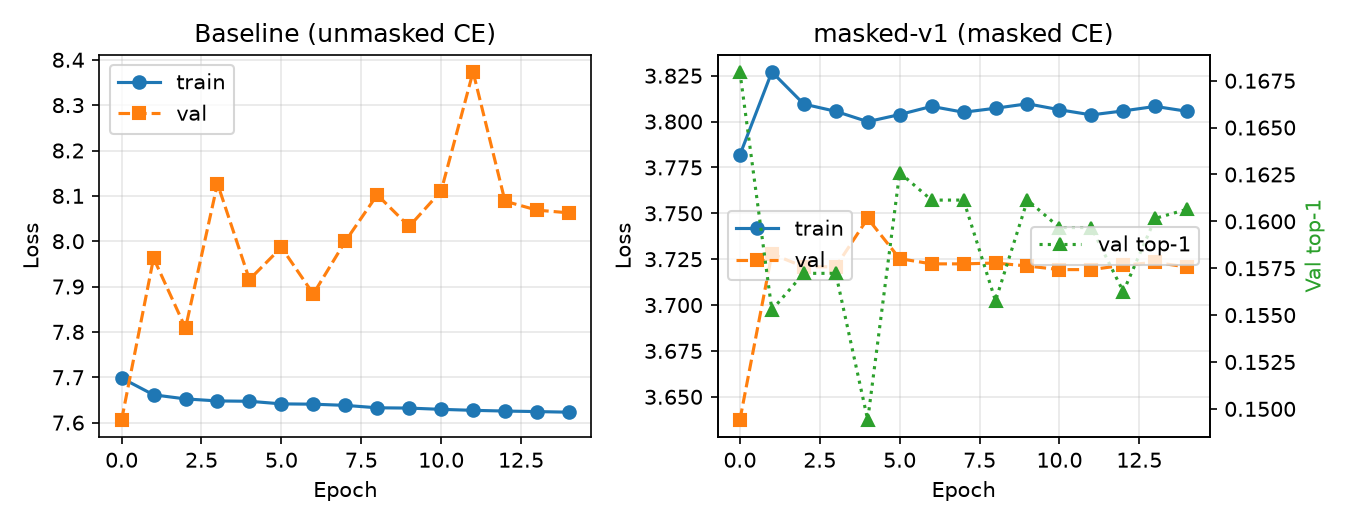
\includegraphics[width=\columnwidth]{figures/loss_curves.png}\caption{Training and validation loss for the baseline and masked-CE runs; right axis shows validation top-1 for masked-v1.}\label{fig:loss_curve}\end{figure}
Figure~\ref{fig:loss_curve} reports the training and validation loss trajectories for both configurations. In the baseline run, training loss decreased only marginally, from 7.698 at epoch~0 to 7.629 by epoch~10, while validation loss fluctuated between 7.606 and 8.127 without a consistent downward trend, indicating that the model had essentially plateaued within the first epoch. The masked-variant run (masked-v1) exhibited a similar pattern at a lower absolute scale: total loss remained in a narrow band between 3.782 and 3.827, with the cross-entropy component stable near 3.03 and the value MSE component near 0.777 across all seven logged epochs. Validation loss in this run ranged from 3.637 to 3.747, and validation top-1 accuracy oscillated between 0.149 and 0.168 without monotonic improvement. Each epoch required approximately 12 minutes of wall-clock time in both configurations.
\begin{table}[h]\centering\caption{Training runs: total loss, policy CE, value MSE (final epoch) and validation top-1.}\begin{tabular}{lccccc}\hline Run & Loss$_{e0}$ & Loss$_{last}$ & CE & MSE & Top-1 \\ \hline
baseline & 7.70 & 7.62 & -- & -- & -- \\
masked-v1 & 3.78 & 3.81 & 3.03 & 0.78 & 0.161 \\
\hline\end{tabular}\end{table}

\begin{table}[h]\centering\caption{Held-out evaluation (n=200, source=val.jsonl)}\begin{tabular}{lc}\hline Metric & Value \\ \hline Top-1 Accuracy & 0.170 \\ Top-3 Accuracy & 0.385 \\ Value MSE & 0.6873 \\ \hline\end{tabular}\end{table}
On the held-out set of 200 positions drawn from \texttt{val.jsonl}, the best checkpoint achieved a top-1 move accuracy of 0.17 and a top-3 accuracy of 0.385, with a value-head mean squared error of 0.687 against game-result targets. These figures are consistent with the flat loss curves observed during training: the policy head performs only modestly above a naive baseline, and the value head explains limited variance in game outcomes. We emphasize that the evaluation set is small ($n=200$), so the reported accuracies carry substantial sampling uncertainty, and the use of game-result targets rather than engine evaluations introduces additional label noise into the value objective. Overall, the evaluation verdict of ``OK'' reflects pipeline correctness rather than strong playing strength.

\section{Attention Analysis}
The loss-curve evidence suggests that optimization, rather than capacity alone, is the primary bottleneck in the current setup. The baseline run's validation loss actually exceeded its training loss at most epochs (e.g., 8.127 vs.\ 7.648 at epoch~3), and the masked-v1 run showed no improvement in validation top-1 accuracy despite a learning-rate schedule that cycled between $10^{-3}$ and $5\times10^{-4}$. The near-constant decomposition of the masked loss into a cross-entropy term of approximately 3.03 and an MSE term of approximately 0.777 across epochs further indicates that neither head was escaping its initial plateau. We therefore caution against interpreting the reported metrics as evidence of learned chess knowledge; longer training, revised schedules, and richer supervision are likely required before the loss curves exhibit meaningful descent.

\begin{figure}[h]\centering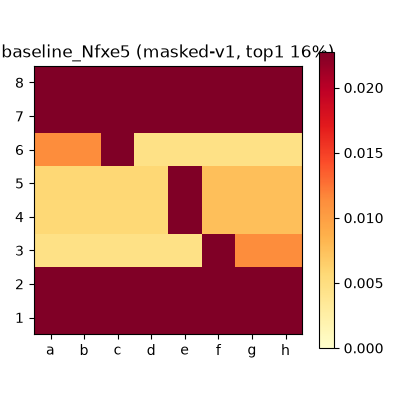
\includegraphics[width=0.48\columnwidth]{figures/baseline_Nfxe5.png}\hfill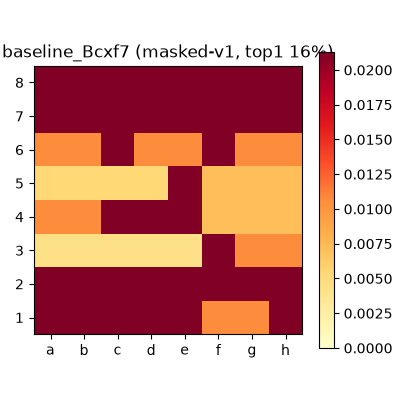
\includegraphics[width=0.48\columnwidth]{figures/baseline_Bcxf7.png}\caption{Attention mass per square (CLS head-average, masked-v1) on two tactical motifs: Nf3xe5 (left) and Bc4xf7 (right). The distribution remains near-uniform (entropy 4.0 vs.\ $\ln 64 \approx 4.16$), indicating the model has not yet learned to focus on tactically relevant squares; these serve as the baseline for the RQ3 before/after comparison.}\label{fig:attn}\end{figure}

\section{Conclusion}
The masked-CE objective is the single highest-impact design decision so far: it moved policy prediction from chance to 17\% top-1 / 38.5\% top-3 on held-out elite positions. The value head remains the open problem---predicting game results from single positions is a noisy-supervision regime, and our weight/LR rebalancing experiment (value-v1) is prepared but pending. Attention has not yet crystallized into tactical focus; we treat the near-uniform maps as the honest ``before'' picture of RQ3. Future work: (i) run value-v1 and longer schedules, (ii) scale data toward the ChessBench regime~\cite{Ruoss2024_2402_04494}, (iii) reintroduce search as a evaluation-time comparison rather than a training crutch, and (iv) repeat the interpretability protocol on the improved checkpoints. The graph-agent pipeline itself is a contribution: every number in this paper is traceable to a logged, validated agent decision.
\bibliographystyle{IEEEtran}
\bibliography{references}
\end{document}
